\chapter{State of the Art}
\label{cha:StateOfTheArt}

To answer the posed questions (see chapter \ref{cha:Introduction}), the attention during research was directed to pose estimation of articulated objects. A majority of the selected reference papers focus on the pose extraction of a human body. Depending on the approach different steps are required which can be generally subdivided into the digitalization of the object to be captured (see subsection \ref{sec:reconstruction}) and its segmentation into rigid parts (see subsection \ref{sec:segmentation}). Regardless of the chosen approach many difficulties have to be overcome in order to estimate the joints and skeleton. A key role of the pose estimation method constitutes the registration of surfaces (see section \ref{registration}). It is commonly referred to as an optimization problem as the goal is to detect the best possible outcome.
%
\begin{figure}[H]
	\centering
	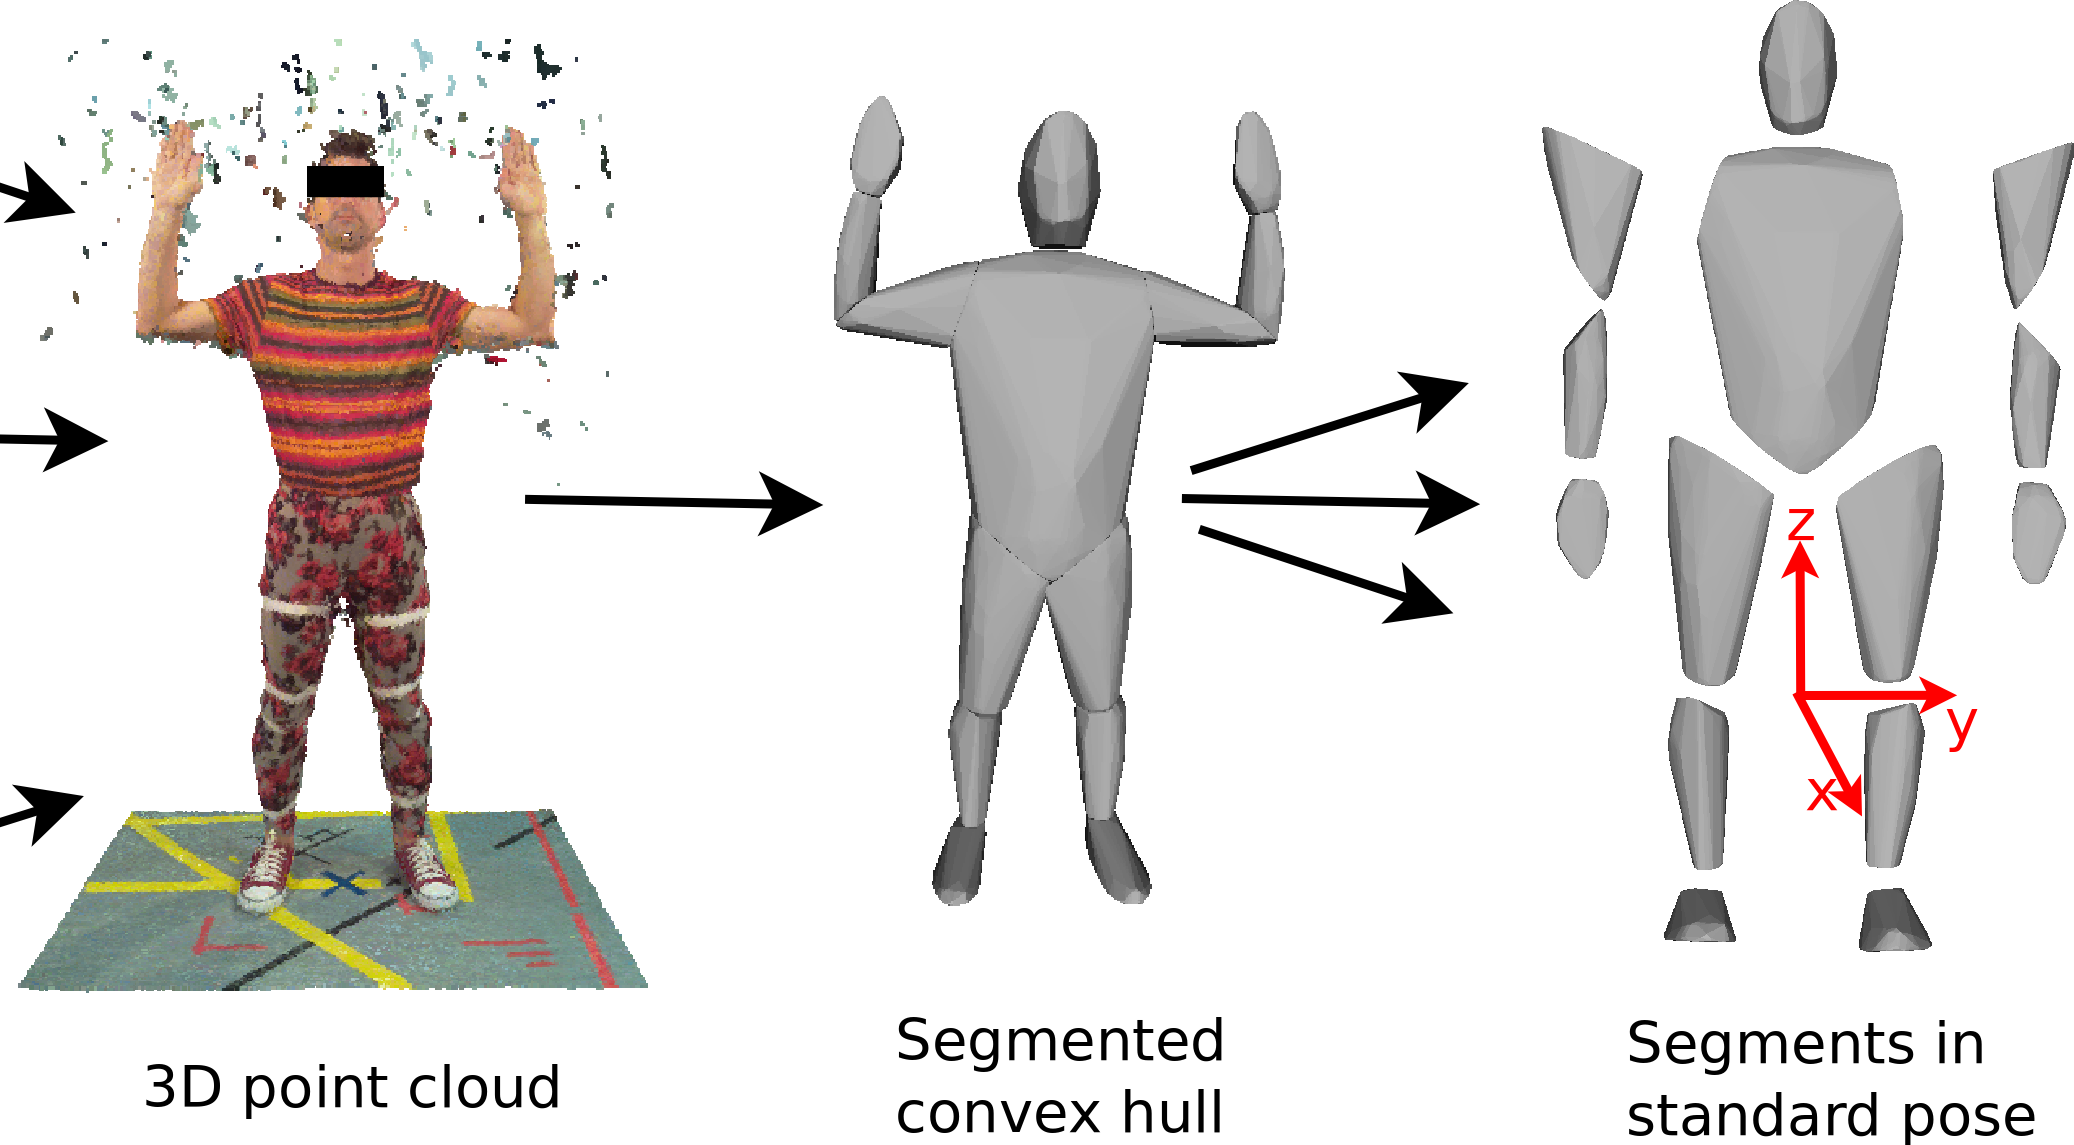
\includegraphics[width=0.7\linewidth]{reconstructionWorkflow}
	\caption{General pose estimation approach. As a first step the captured object needs to be digitalized (a) and if required reconstructed(b) to a mesh. Then, it needs to be segemented into its rigid parts (c) which is the key part in order to estimate the joints and skeleton.}
	\label{fig:posecapture}
\end{figure}
%
%TODO: new image with puppet! --> picture, point cloud, skeleton
%
\section{Surface Registration}
\label{registration}
Generally, registration in computer vision and computer graphics refers to the alignment of overlapping components of two or more digital data sets \cite{survey}. Thereby, the most essential part is the detection of point correspondences between two surfaces to be registered often supported by RANSAC \cite{ransac}. One main application is the alignment of two or more incomplete range scans of an object from different view ports to obtain a complete model. Further applications are symmetry detection, articulation of non-rigid objects and subpart identification. For this reason a vast number of pose estimation and skeleton extraction approaches rely on a successful registration. 

\subsection{Functionality}
A discrimination between rigid and non-rigid registration can be done. In the former case, it is assumed that two surfaces are related by a rigid transformation which can seen on figure \ref{fig:registration}~(a). A well-known approach for a rigid registration is the iterative closest point (ICP) \cite{ICP}. It requires a similar initial position of two shapes to avoid a local optimum. For this purpose it is often taken advantage of the principal component analysis (PCA) \cite{pca} of shapes. With each iteration step the point correspondences between two input objects are updated by selecting the closest points. As a next step, the rigid transformation between two shapes is recalculated considering the detected correspondences. A matching error $e$ is achieved, which states the total euclidean distance between the associated points of the registered shapes. The algorithm terminates after a predefined number of iterations or if a specified value for $e$ is achieved. Considering two non-rigid surfaces composed of rigid parts (e.g. a human), the rigid registration will not lead to a convincing result as the individual rigid parts may undergo varying rigid transformations. In this case a non-rigid registration is required, which performs a segmentation into rigid parts which can be seen on figure \ref{fig:registration}~(b).
%
\begin{figure}[H]
	\centering\small
	\begin{tabular}{cc}
		\fbox{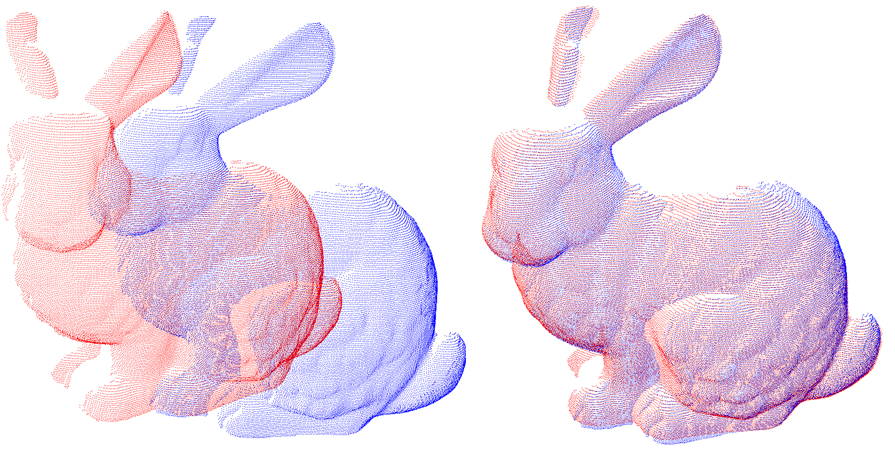
\includegraphics[width=0.43\textwidth]{stanfordBunny}} &
		\fbox{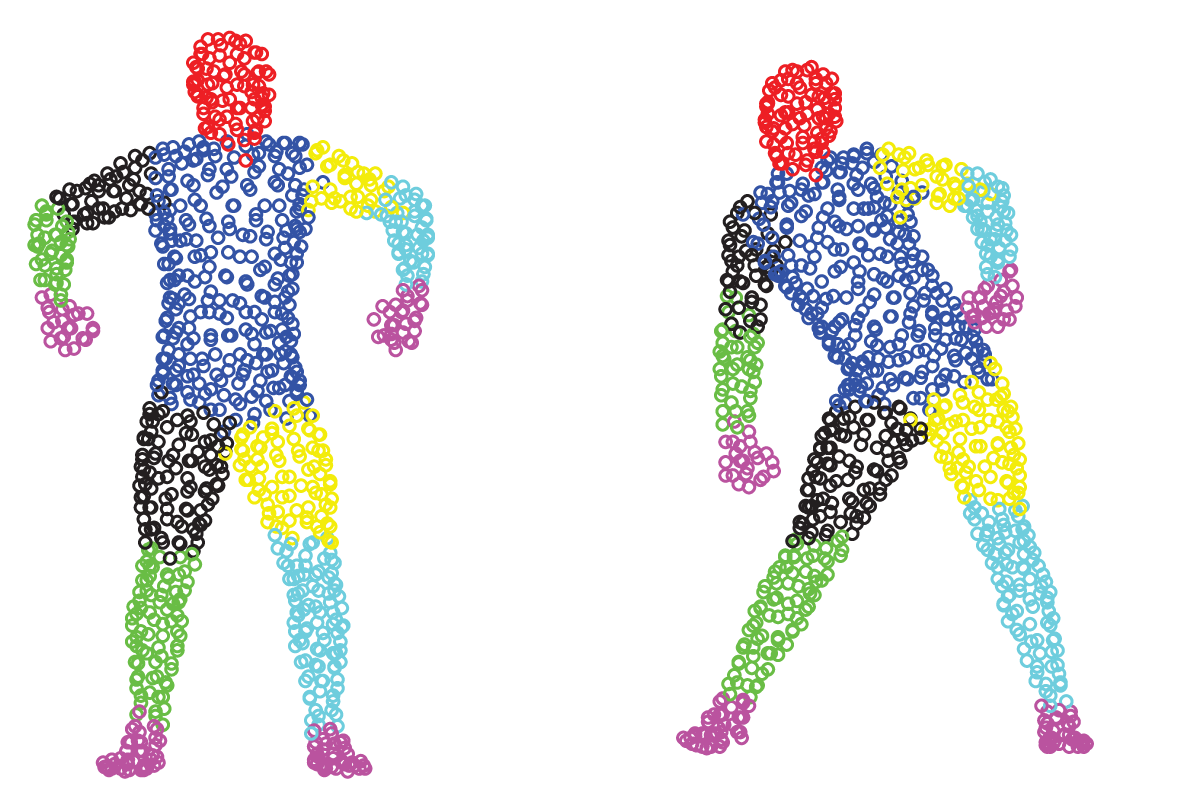
\includegraphics[width=0.45\textwidth]{nonrigidregistration}} 
		\\
		(a) & (b) 
	\end{tabular}
	\caption{Rigid registration of a rigid model of the stanford bunny~(a) \cite{stanfordBunny} and non-rigid registration of a human~(b) \cite{registrationHuman} composed of several rigid parts.}
	\label{fig:registration}
\end{figure}\textbf{}
%

\subsection{Difficulties}
Some factors complicate the accomplishment of a visual successful registration. Main difficulties are noisy data and outliers which often arise from low resolution scans. Furthermore, there might only be a limited number of overlapping data which is the case for multiple incomplete scans of an object from different view ports. Self occlusion and variations form initial poses are influence factors which should not be underestimated. In case of non-rigid registration the main difficulty is the establishment of correspondences as several transformations of the data need to be considered. To generally reduce the correspondence space specific constraints can be set. Those include for example the computation of point features, which are quantities that add additional information to a point besides its coordinates. Correspondences between two shapes can then be computed by feature matching. Also saliences plays a major role for correspondence detection, which are represented by points being considerable different from neighbors. By placing markers on the object or assuming topology, the allocation of points to rigid parts can be simplified. Also the prior information of articulation places a valuable contribution as no deformations have to be considered. 
One main drawback of the non-rigid registration is that it is computationally expensive and time-consuming, as the corresponding body parts of two shapes need to be detected iteratively. Additionally, the inevitable difficulty of finding the global optimum related to ambiguous body parts is present.

\subsection{Optimization}
Several optimization approaches are proposed to overcome some of the stated difficulties. One established method regarding the detection of correspondences is the Expectation-Maximization (EM) which alternates between two steps: detecting correspondences and optimizing the transformation. To avoid local minima a global optimization can be pursuit, for example by forming a decision tree. Furthermore, stochastic optimization take into account statistics and probabilities. Popular related methods apply voting and belief propagation, such as Markov random fields (MRF). 
%
\section{Pose estimation of articulated objects}
\label{poseEstimation}

%TODO write about history? What has been done, what will come? 

To successfully estimate the pose of an articulated object, generally two main parts have to be performed: the digitalization of the object and the segmentation of the data into rigid parts. Although 3D scanner are getting more and more common, pose estimation from 2D images gets more and more important. This thesis focuses on the segmentation of the input data into rigid parts, therefore the digitalization of the object will not be covered in detail.

\subsection{Digitalization of the object}
\label{sec:reconstruction}
As a first step the object to be captured needs to be digitalized for the subsequent segmentation step. By a scanning step the real shape is collected as 2D or 3D data. The raw data in form of 2D images, video streams, or even point clouds in 2D or 3D can be directly used for pose estimation. Multiple commercial 3D scanner are available strongly varying in precision and resolution and purchase price. Especially, RGB-D sensors have taken on greater significance for 3D reconstruction !!!REF KINECT!!! as they are easily accessible and inexpensive. Usually, a subsequent reconstruction step is performed which converts the raw data into a mesh often combined with registration of different scans. Reconstruction from images and videos gets more and more popular as they are independent from expensive scanner. !!!REF
Voxelization, Shape from Silhouette, Shape from Shading, 2d images!!! Some approaches also skip the digitalization step and take a 3D mesh as input from a modeling software. Shape from silhouette \cite{mocap}
%
%TODO: add scanning/reconstruction methods
%
\subsection{Segmentation}
\label{sec:segmentation}

The crucial computer vision part of the pose estimation is the segmentation of the digitalized object into its rigid parts in order to estimate joints and the skeleton. The main idea is to allocate each data point of an input object to a rigid part. For that, additionally to the input data any kind of prior information is indispensable. Regarding the non-rigid registration the same object in another configuration is required which is usually referred to as a \textit{template}. Generally the segmentation approaches are then classified into supervised (see section \ref{supervised}) and unsupervised methods (see section \ref{unsupervised}) whereby the former depends on manual user input. 

\section{Supervised methods}
\label{supervised}

Supervised methods for pose estimation greatly simplify the segmentation procedure as certain assumptions of the object can be made. Examples include the placement of markers on the real object or the digitalized model to label its joints linking the rigid parts (see \cite{hierarchicalMethod} and \cite{estimatingConfigurations}). Furthermore, the usage of an \textit{object model} is frequently employed to have prior knowledge of the number of rigid parts and possibly the length and shape of an object (see \cite{hierarchicalMethod} and \cite{mocapShapeFitting}). Another well known approach uses the motion information of known point correspondences from image sequences (see \cite{segmentationMotion}, \cite{animatedObjects}). The approach from \cite{sfsMocap} sequentially estimates each joint by the person being captured moving one body part at a time. By extracting and registering the resulting CSPs (colored surface points) a joint can be estimated which can be seen on figure \ref{fig:supervisedMotion}. 
%%

%TODO: add important references
%TODO: add picture of csp

\begin{figure}[H]
	\centering
	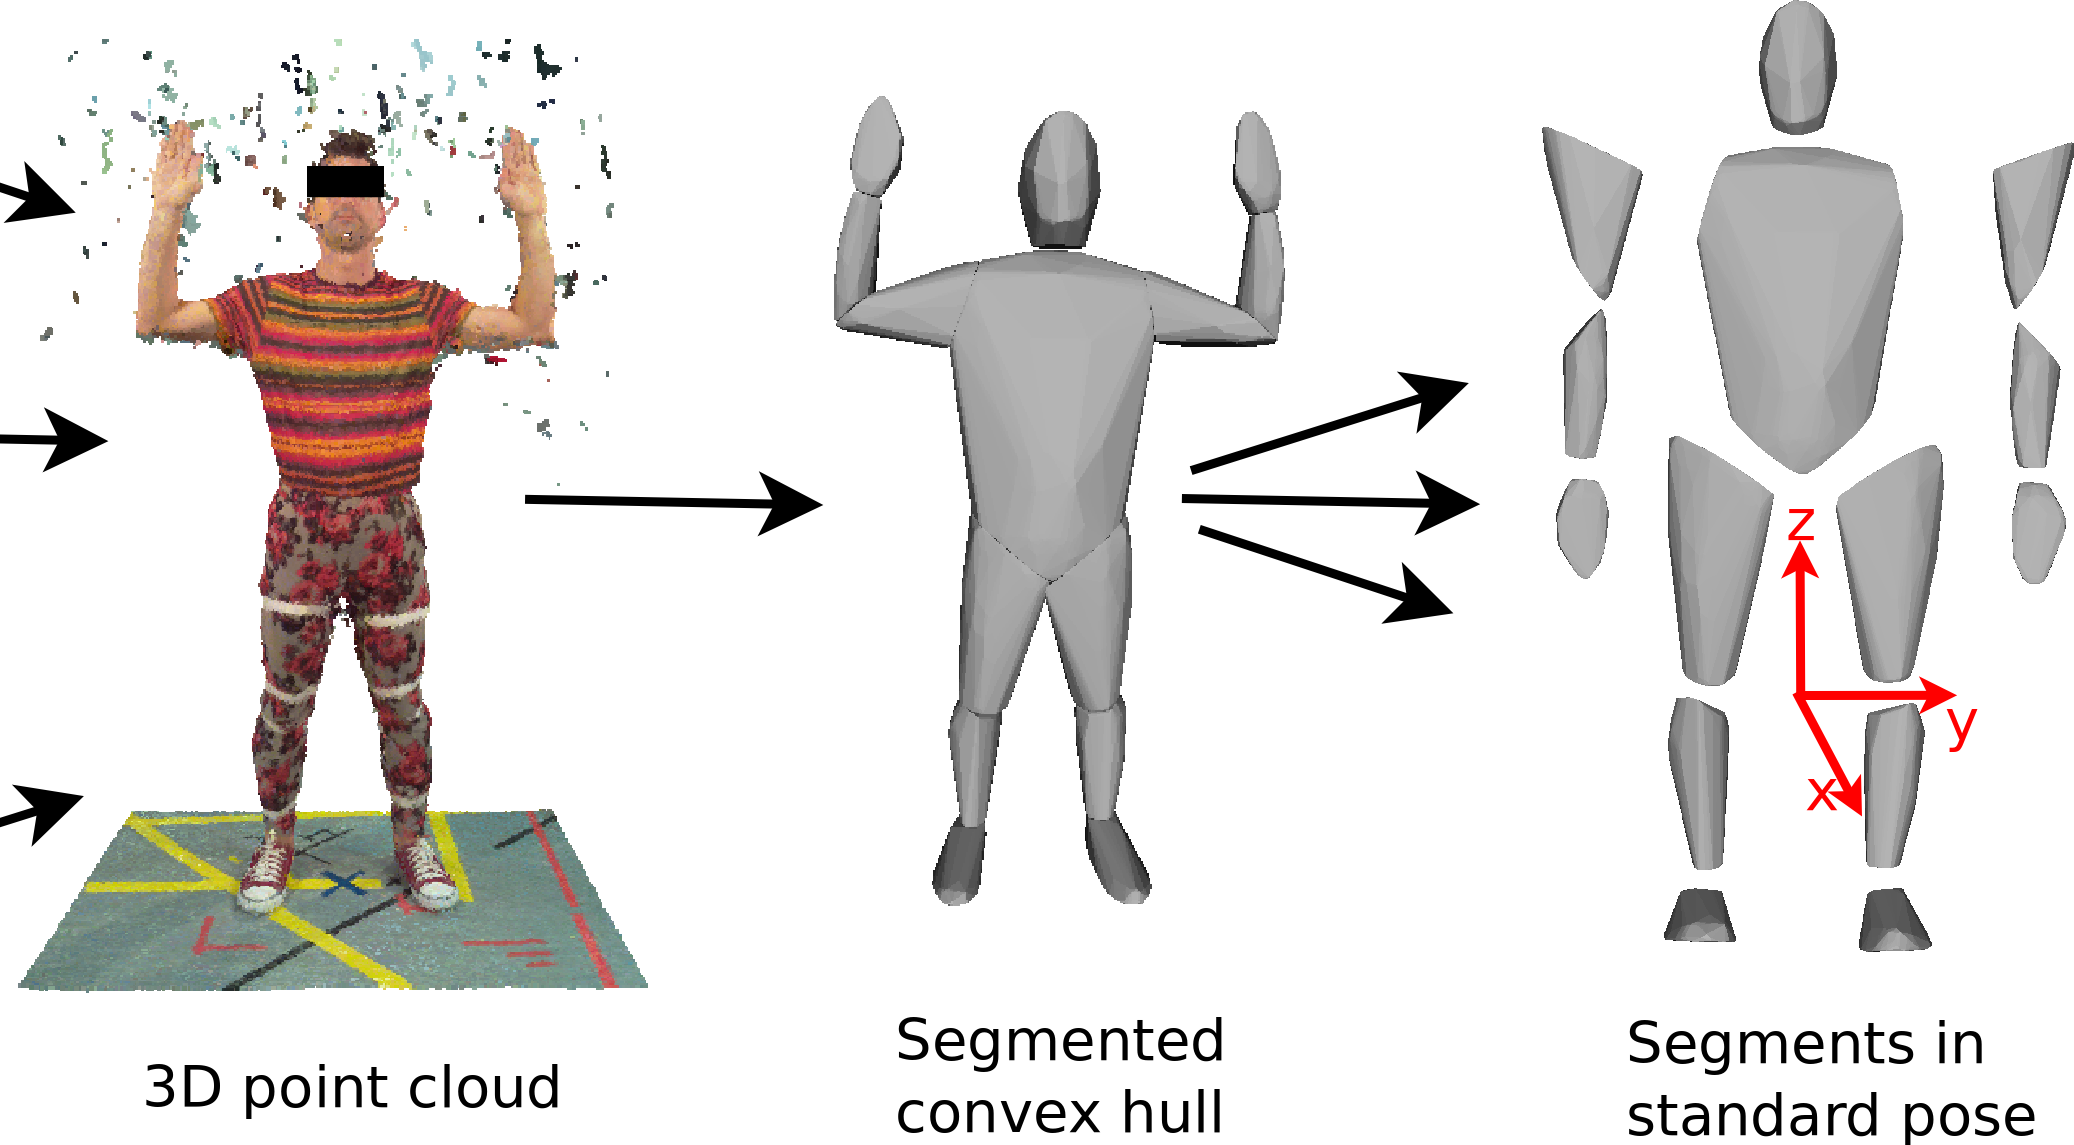
\includegraphics[width=0.7\linewidth]{reconstructionWorkflow}
	\caption{General pose estimation approach. As a first step the captured object needs to be digitalized (a) and if required reconstructed(b) to a mesh. Then, it needs to be segemented into its rigid parts (c) which is the key part in order to estimate the joints and skeleton.}
	\label{fig:supervisedMotion}
\end{figure}
%%
Further approaches take advantage of training data and machine learning to estimate the pose of a human. The approach from \cite{consensusvoting} uses a convolutional neural network to train a key point detector on 2D images. 

\section{Unsupervised methods}
\label{unsupervised}

Although the supervised pose estimation approaches from subsection \ref{supervised} result in promising results they depend on manual user input to be specified before the segmentation. Thus, they are either time consuming, inconvenient and or restrict themselves to specific articulated objects (e.g. humans). Therefore, unsupervised methods are proposed that work independent from user inputs and are therefore applicable for unknown articulated objects without having prior knowledge about its rigid parts. The proposed methods only require an articulated object in two different configurations as input, no prior information about the object's topology have to be provided. As those assumptions conform to the goal of this thesis, all reference paper are listed under related work (see subsection \ref{relatedWork}). 
%%

\subsection{Related work}
\label{relatedWork}

A main approach for non-rigid registration is proposed by Anguelov \cite{Anguelov04} applying the correlated correspondence algorithm \cite{CorrelatedCorrespondance}. The algorithm takes a \textit{template} Mesh of an object $M_0$ and any number of Meshes of the same object $M_1,\ldots,M_n$ in different configurations as input. The algorithm then performs a Markov Network with loopy belief propagation and Expectation-Maximization to iterate between finding a decomposition of the \textit{template} into rigid parts and detecting them in the other meshes. Thereby, it takes advantage of PCA and the ICP. Furthermore, a random clustering is applied to facilitate the detection of associated rigid parts (see figure \ref{fig:correlatedcorrespondance}).
%%
\begin{figure}[H]
	\centering
	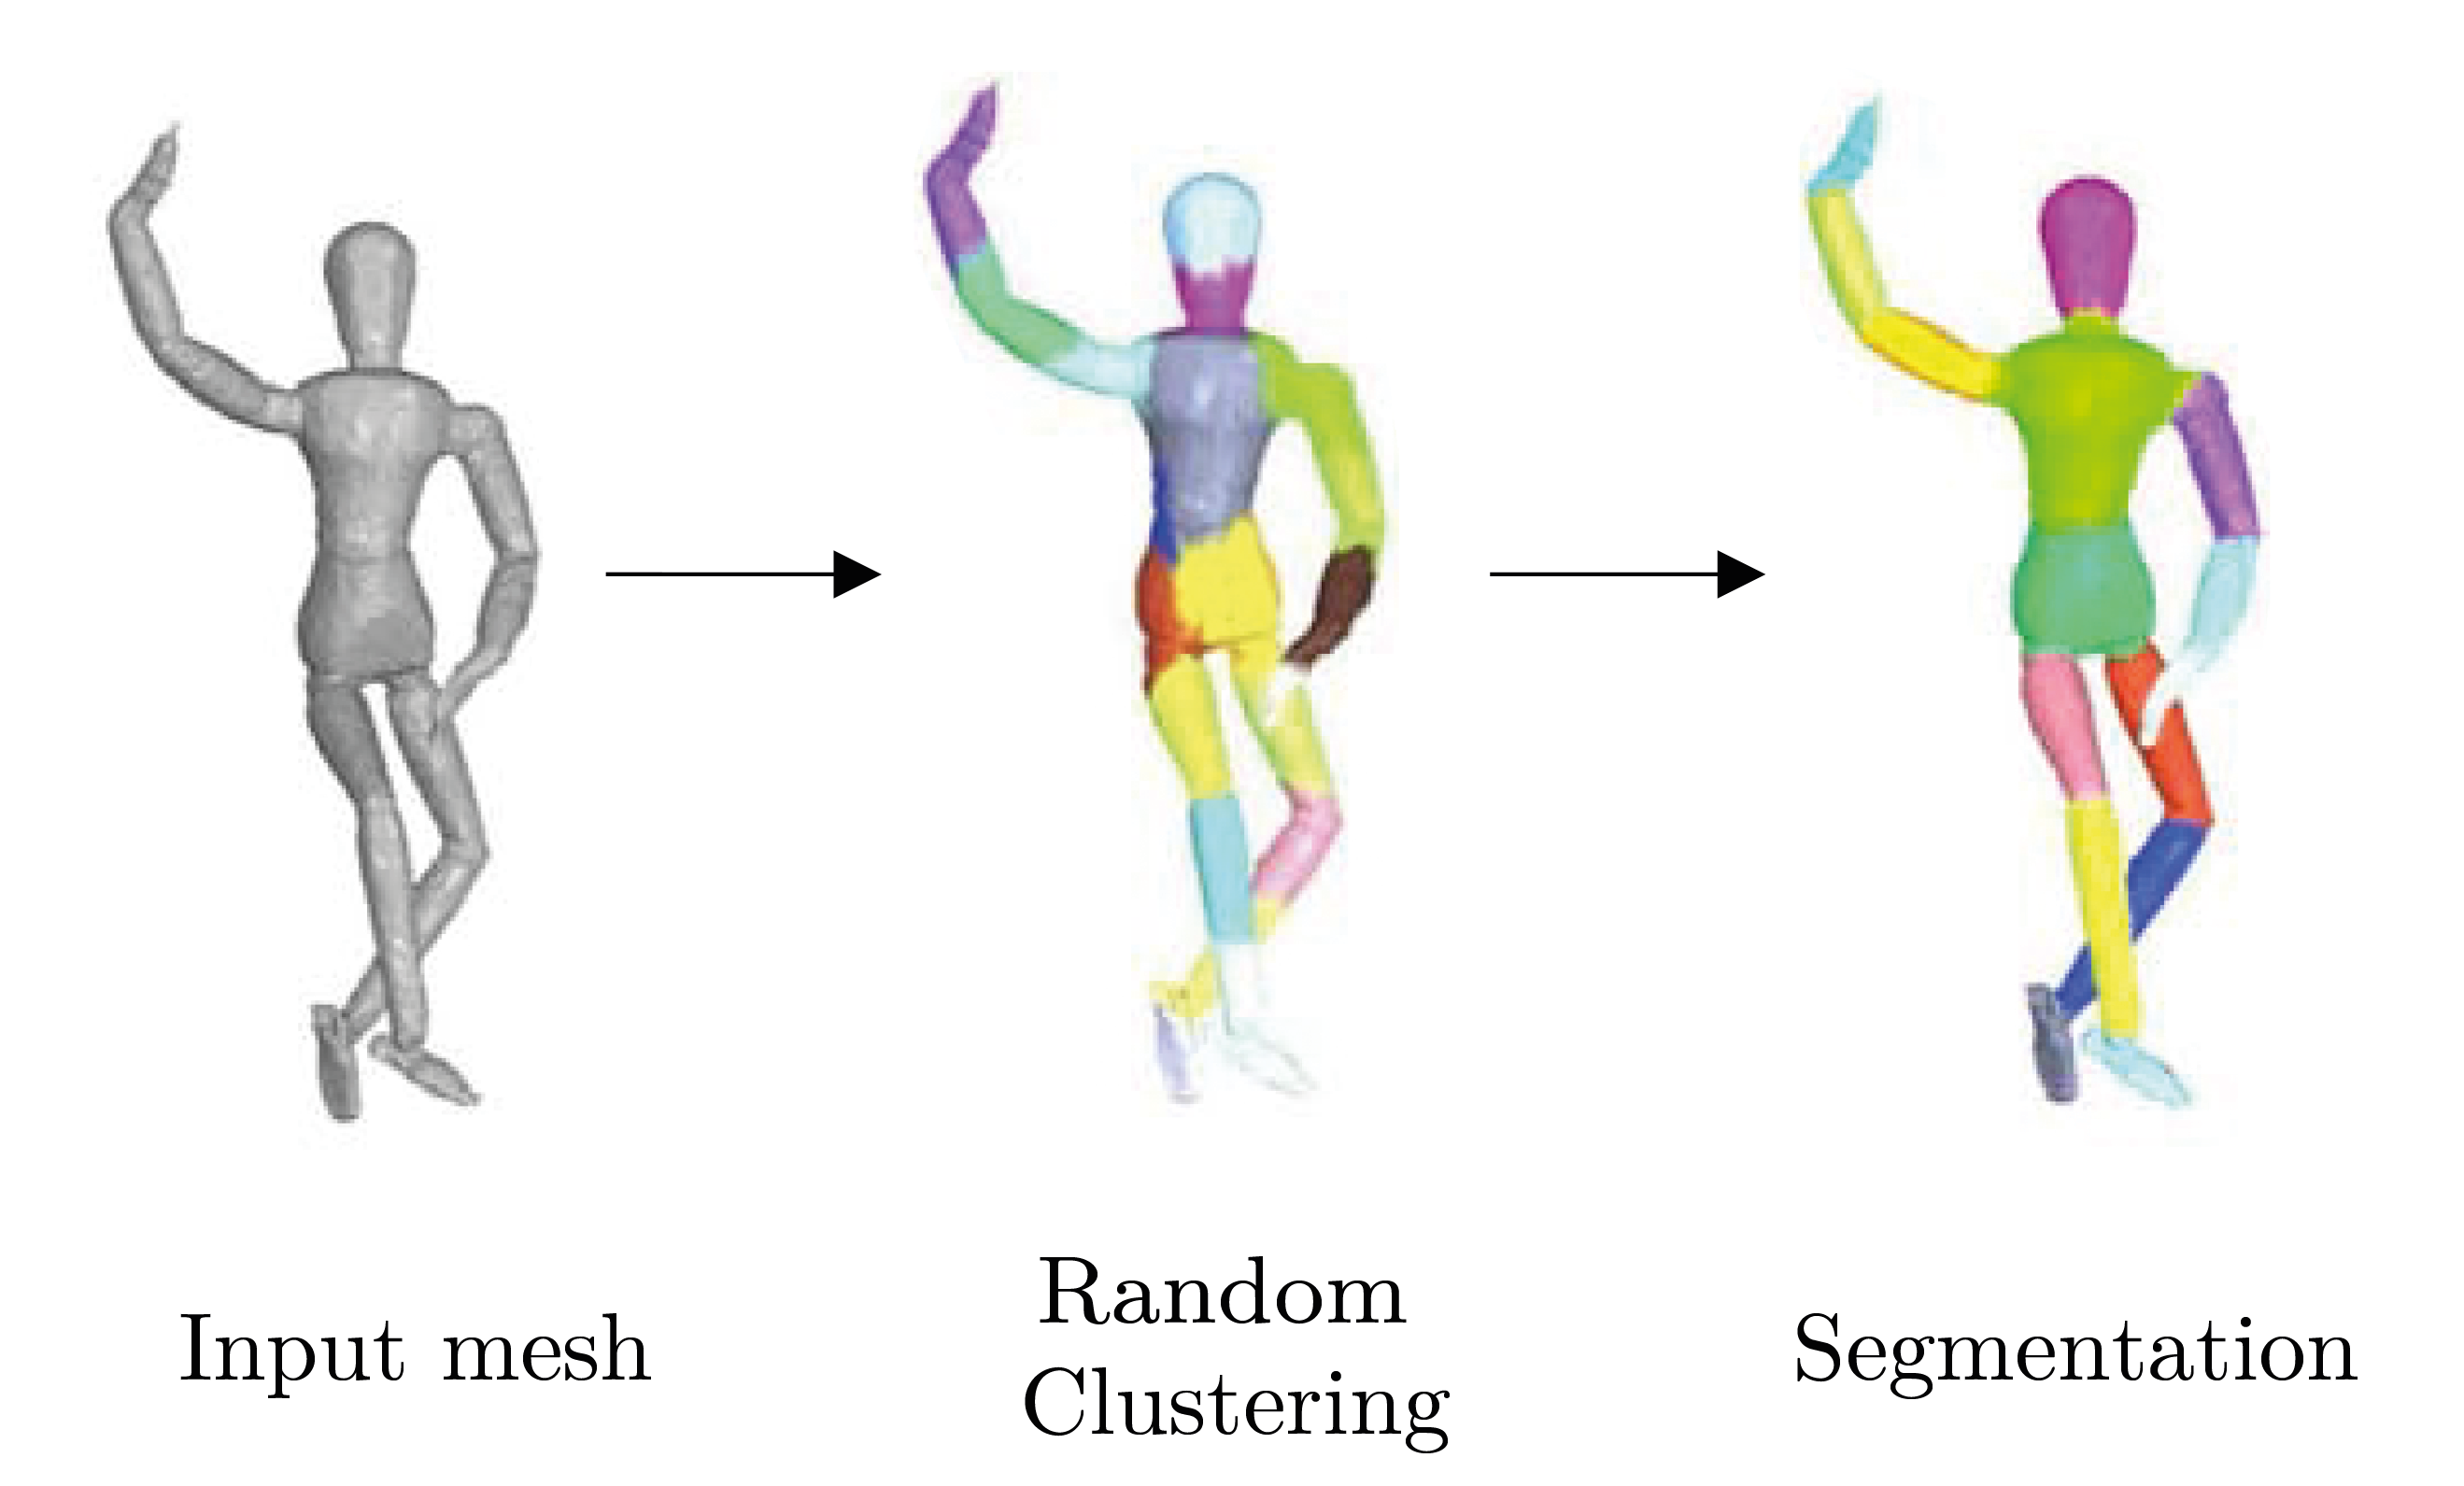
\includegraphics[width=0.7\linewidth]{anguelov}
	\caption{Segmentation a template mesh $M$ into its rigid parts by applying random clustering and a probabilistic framework to iteratively detect associating parts in another mesh \cite{Anguelov04}.}
	\label{fig:correlatedcorrespondance}
\end{figure}
%%
Another approach proposes the recursive detection of body parts by the \textit{LRP} -- ``largest rigid part'' algorithm \cite {guo2016correspondence}. It discovers the articulated parts of two objects in different configurations by initially detecting the largest rigid part. It is represented as the biggest overlapping point cluster by applying a single rigid transformation. To achieve that, sparse correspondences with feature matching in combination with RANSAC are implemented. Proceeding from a detected ``largest rigid part'',linking parts are recursively detected by growing clusters reapplying the algorithm on unclustered points (see figure \ref{fig:LRP_algorithm}).
%%
\begin{figure}[H]
	\centering\small
	\begin{tabular}{cc}
		\fbox{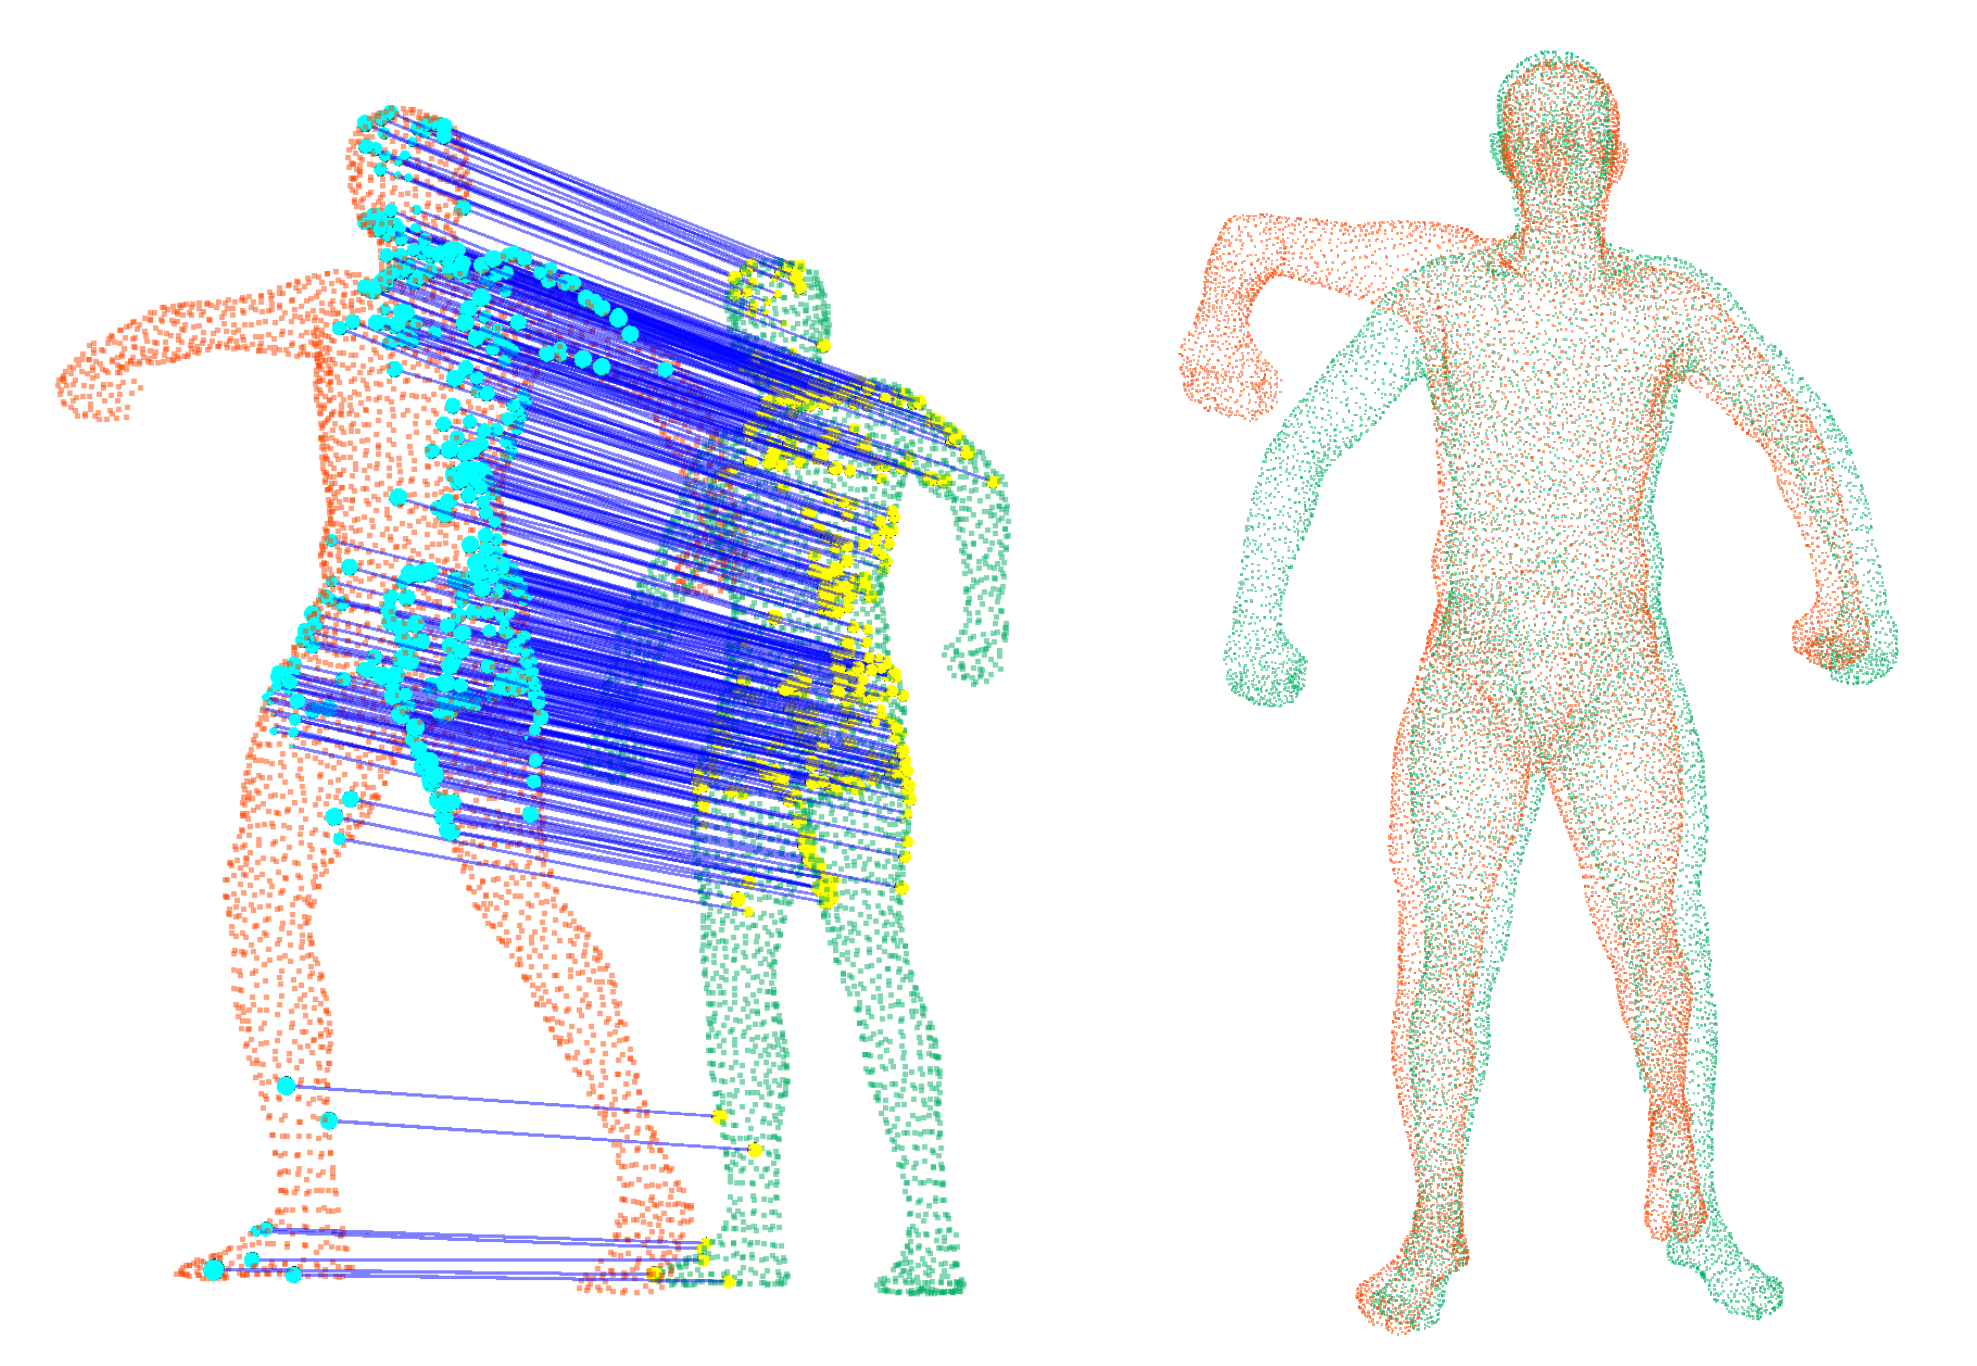
\includegraphics[width=0.45\textwidth]{LRP_body}} &	
		\fbox{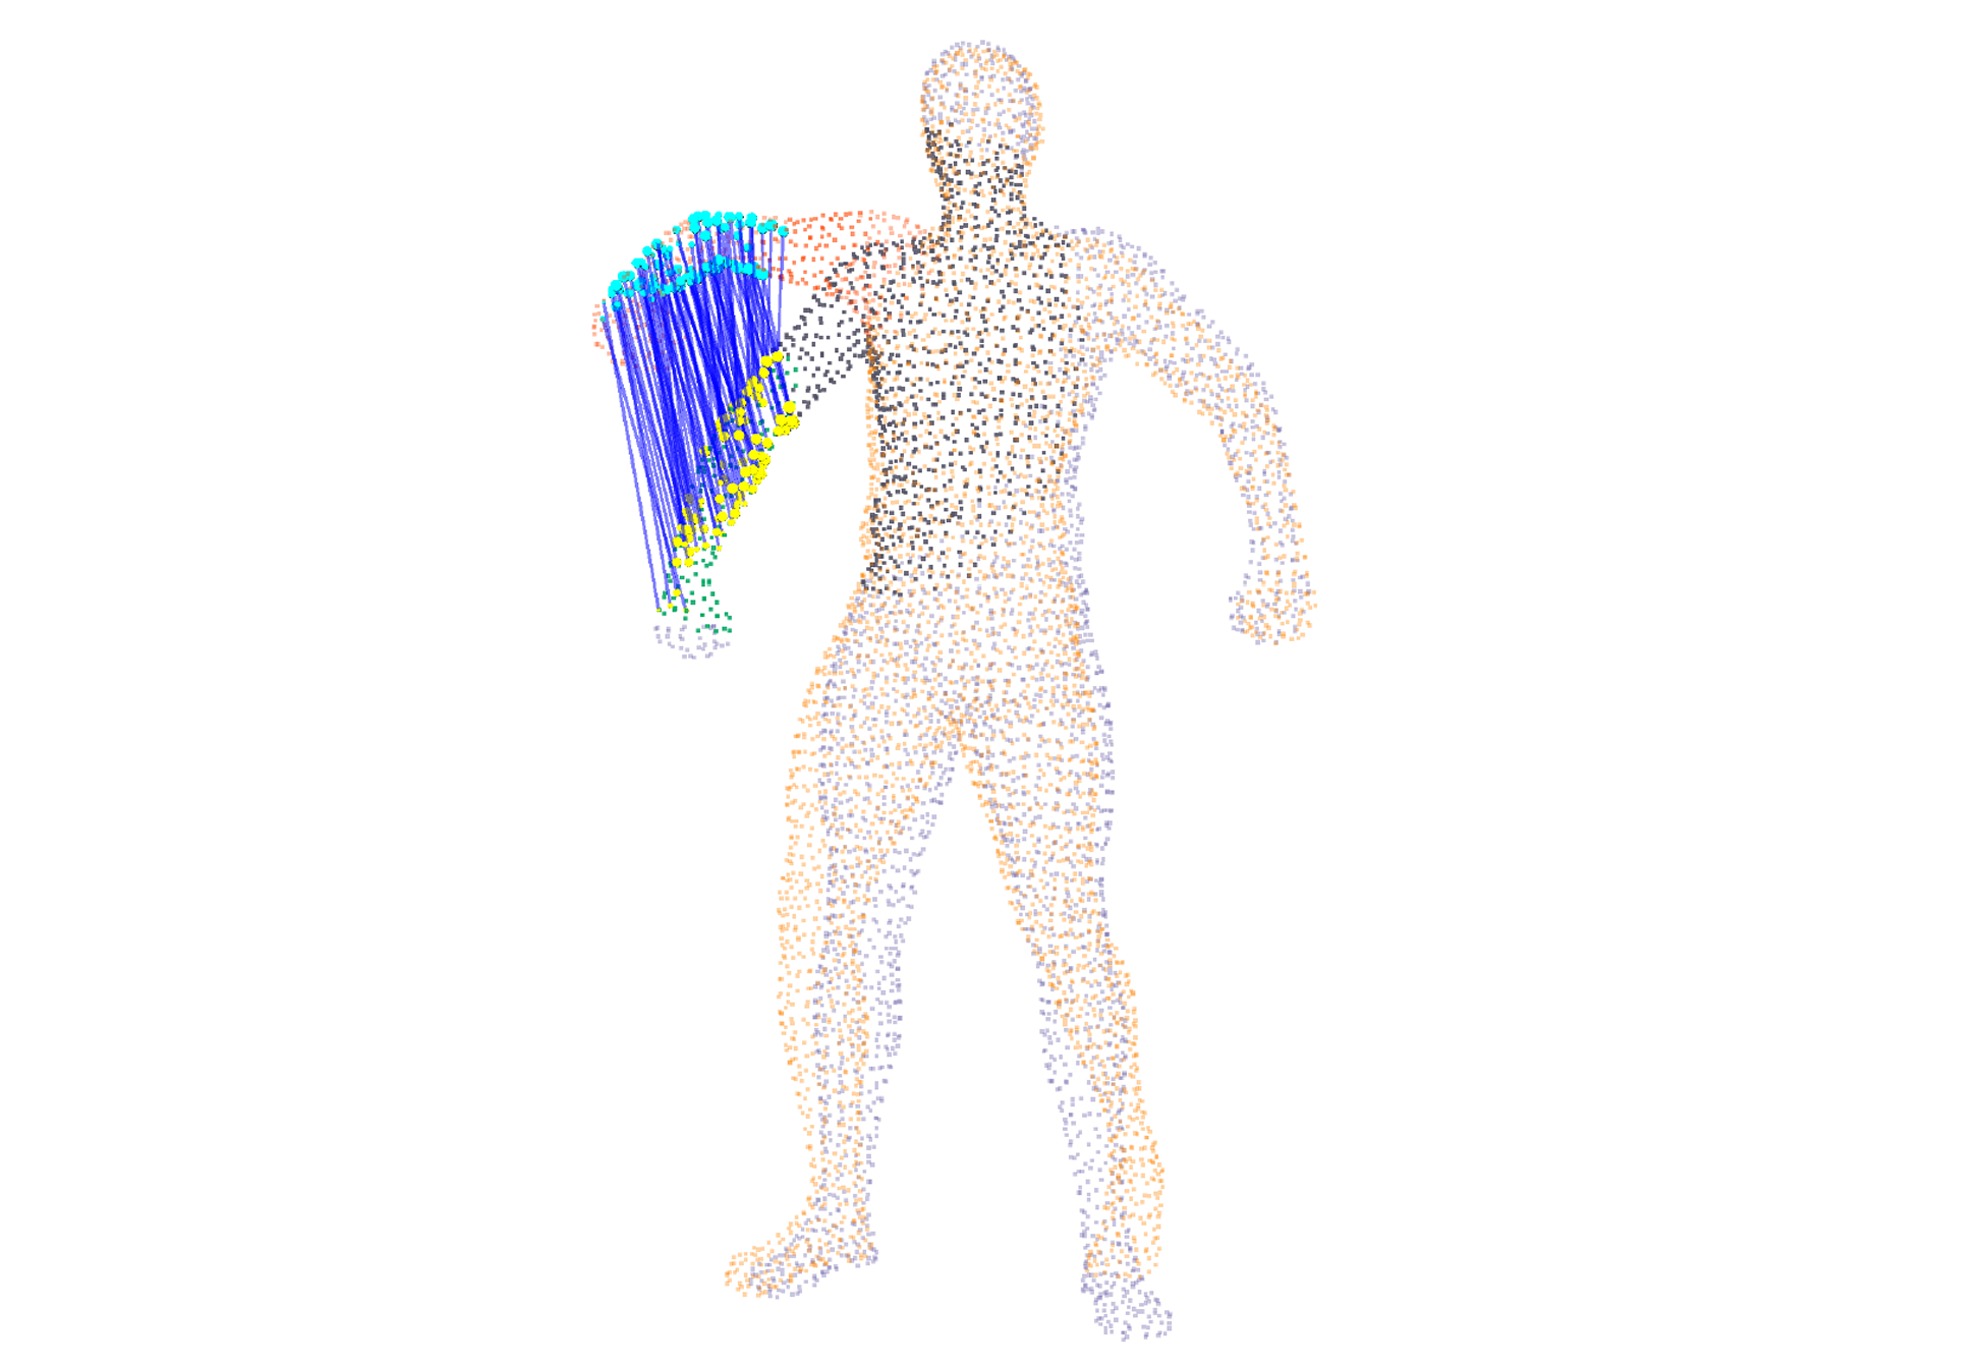
\includegraphics[width=0.45\textwidth]{LRP_arm}} 
		\\
		(a) & (b) 
	\end{tabular}
	\caption{Detecting the largest rigid part of an object~(a), and align the object to recursively detect linking parts to the LRP~(b) \cite{guo2016correspondence}.} 
	\label{fig:LRP_algorithm}
\end{figure}
%%
Chang et al \cite{chang08articulated} developed an approach for the alignment of articulated shapes from range scans with missing data in different poses. They sampled the motion of corresponding points by matching feature descriptors of both shapes. The generated motion in form of transformations is clustered to detect the most optimal shape alignment (see figure \ref{fig:motionAlignment}). A related approach by Chang et al proposed skinning weights to the motion and applied Expectation-Maximization to update those weights and the computed transformation \cite{chang09range}.
%%
\begin{figure}[H]
	\centering
	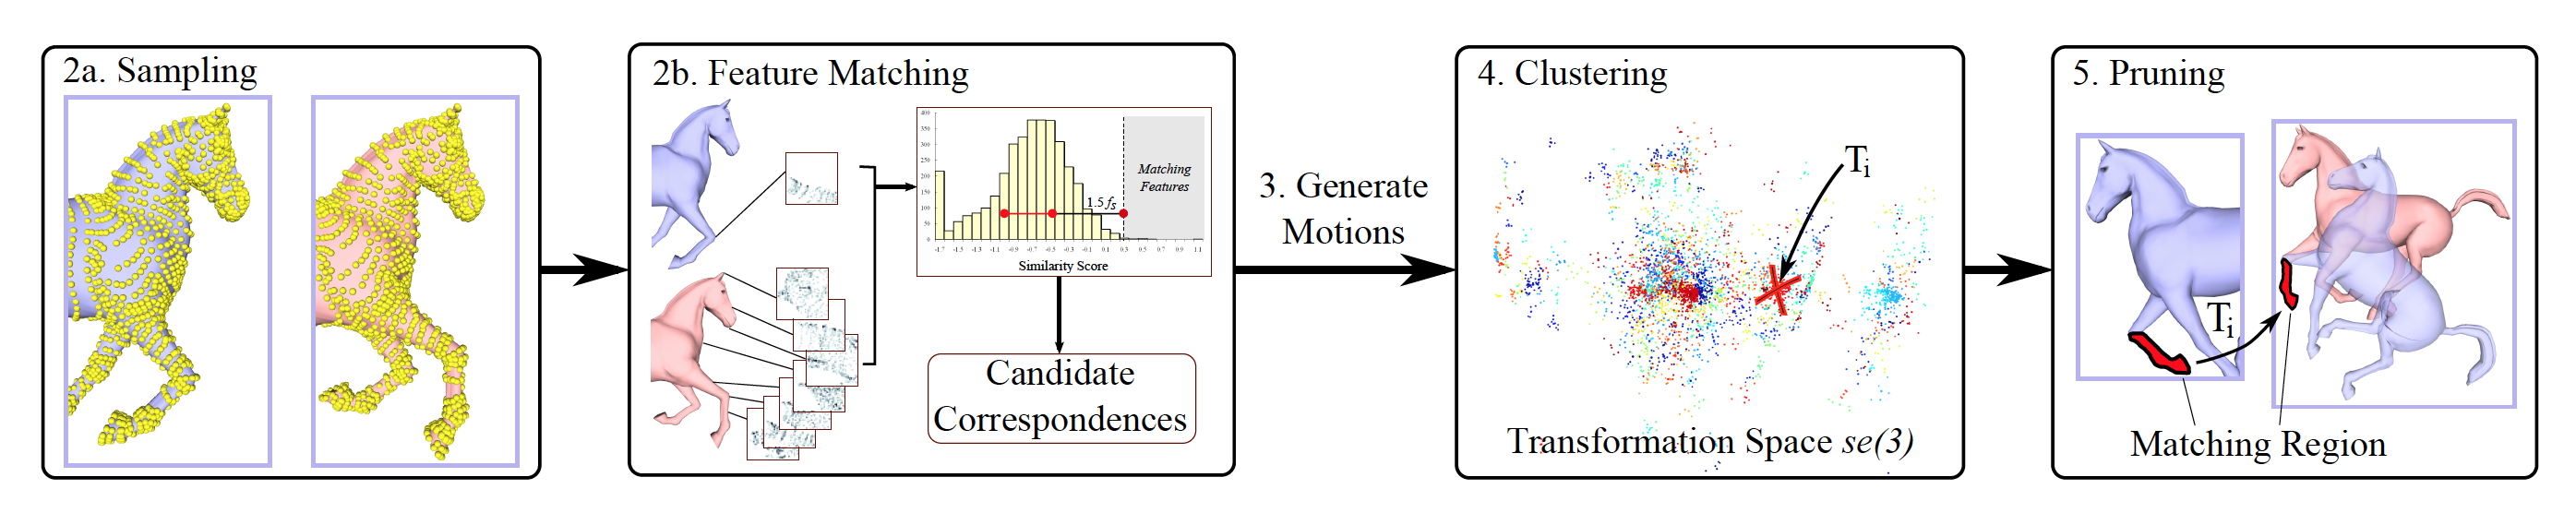
\includegraphics[width=1.0\linewidth]{changMotionAlignment}
	\caption {Alignment of articulated objects in form of range scan by feature matching and clustering of generated motion \cite{chang08articulated}.}
	\label{fig:motionAlignment}
\end{figure}

Another approach is achieved by Symmetrization \cite{Mitra07}, by detecting and aligning the body parts’ symmetry axes of an object(see figure \ref{fig:Symmetrization}). De Goes et al \cite{de2008hierarchical} detect consistent segments from a single pose my computing the diffusion distance of a surface. Another unsupervised method poses the probabilistic registration of articulated human body in form of voxels \cite{probabilisticRegistration}. By fitting splines the input object can be segmented into its rigid parts.

\begin{figure}[H]
	\centering\small
	\begin{tabular}{cc}
		\fbox{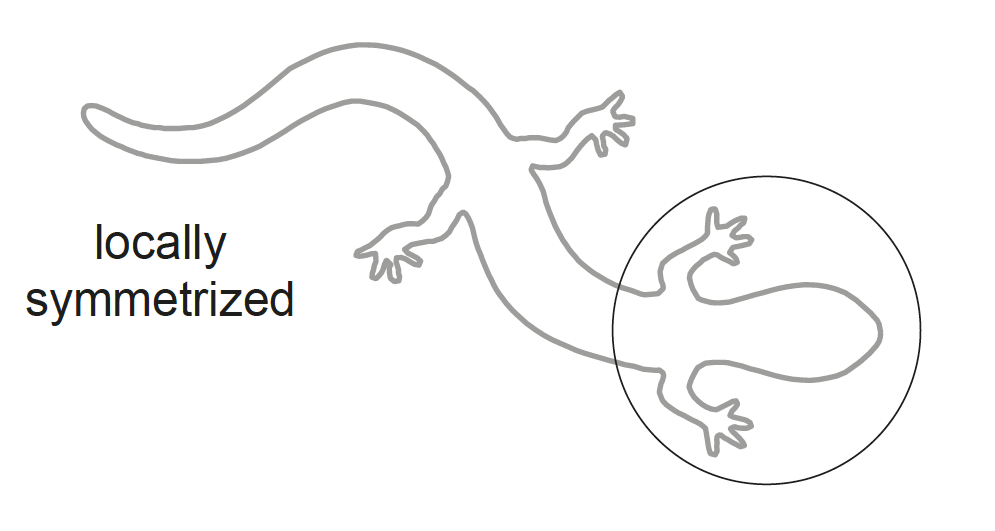
\includegraphics[width=0.45\textwidth]{Symmetrization1}} &
		\fbox{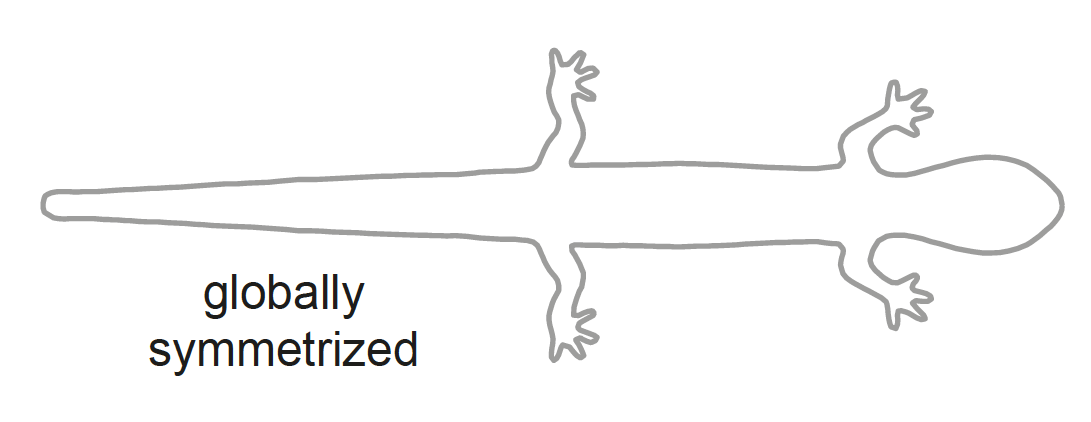
\includegraphics[width=0.45\textwidth]{Symmetrization2}} 
		\\
		(a) & (b) 
	\end{tabular}
	\caption{Detection of the rigid parts of an object by local~(a) and global~(b) Symmetrization \cite{Mitra07}.} 
	\label{fig:Symmetrization}
\end{figure}

%TODO: images?
%%

%TODO: Add other references
\subsection{Main drawbacks}

The proposed approaches achieve convincing results concerning the accuracy of the segmentation and the detection of rigid parts. However, they are all computationally expensive and require a considerable number of computation steps to iteratively detect point correspondences and subsequently rigid parts in two associated objects. This reflects on the run time of the algorithm which offers therefore great potential for improvements e.g. to allow pose estimation in real-time. Taking the existing methods as reference (see section \ref{relatedWork}) two segmentation approaches are proposed. Thereby, the main focus is to reduce the computation steps of the correlated correspondence algorithm \cite{CorrelatedCorrespondance} as well as the LRP algorithm \cite {guo2016correspondence}. To fully focus on the segmentation into its rigid part, the data input in form of 2D point clouds and 2D hulls as well as 3D reconstructions of an articulated object are assumed to be available.